\chapter{From Last Scattering to Baryogenesis}

We begin where Leonard Susskind begins: not with an abstract early-universe mechanism, but with the sky at different distances. Farther out means earlier, and earlier means denser and hotter. From that observational starting point the lecture moves through last scattering, then farther back into pair production and the quark-antiquark soup, then reverses the movie and follows cooling, annihilation, and the tiny fossil asymmetry that survived. These companion notes follow that progression closely and retain selected board evidence from the lecture record prepared with LazyingArt LLC and Video2Book.

\section{Looking Outward Means Looking Backward}

The first move is geometric and observational. We place ourselves at the center and imagine shells at larger and larger distances. Nearby shells show a universe that is scarcely different from the present one. But once we look far enough, the finite speed of light stops being a technicality and becomes the main point: distant means old.

As we look to earlier epochs, the universe becomes denser, and with density comes higher temperature. In the lecture Susskind fixes the picture by an order-of-magnitude comparison: if we look back far enough, we reach a time when the universe was roughly as hot as the surface of the sun. The sky does not \emph{look} like the surface of the sun because the photons have been redshifted on the way to us. At the level needed here, we may summarize the relation as
\begin{equation}
T_{\mathrm{obs}} \sim \frac{T_{\mathrm{emit}}}{1+z},
\end{equation}
and for the last-scattering epoch the lecture uses the rough scale
\begin{equation}
1+z \sim 10^3.
\end{equation}
So the radiation that was emitted from a much hotter environment reaches us with a temperature lowered by about three orders of magnitude.

This opening matters. It means that the early universe is not introduced as a speculative add-on. We are pushed toward it by ordinary observation: to see farther is to see younger, and to see younger is to see hotter matter.

\section{Last Scattering, Ionization, and Opacity}

The first real thermal threshold in the lecture is not baryogenesis but visibility. Hydrogen remains ionized above a temperature of order a few thousand kelvin. Thus when we look back beyond a certain distance we do not find neutral atoms; we find an ionized gas of nuclei and free electrons, together with a large background of energetic photons.

\begin{definition}
The \emph{surface of last scattering} is the transition surface at which the universe changes from an opaque ionized plasma to a transparent gas of neutral atoms.
\end{definition}

The reason for opacity is simple and physical. A plasma is an electrical conductor. Free charges respond to electric fields, slosh back and forth, and re-emit radiation. In that state the universe is not transparent. When the temperature falls below the ionization scale of hydrogen, electrons can bind to nuclei, matter becomes neutral, scattering drops sharply, and the universe becomes transparent.

The lecture treats this as a sudden transition, analogous to the visible surface of the sun:
\begin{align}
T \gtrsim \text{a few}\times 10^3\ \mathrm{K} &\quad \Longrightarrow \quad \text{ionized, opaque},\\
T \lesssim \text{a few}\times 10^3\ \mathrm{K} &\quad \Longrightarrow \quad \text{neutral, transparent}.
\end{align}

That is the observational boundary. Behind it, direct sight gives out. But physics does not give out there. Once the lecture has explained why the universe becomes opaque, it immediately takes the next step: let us go back a little bit further, now by extrapolating with atomic physics, nuclear physics, and particle physics.

\section{Going Further Back: Pair Production and Thermal Thresholds}

At the surface of last scattering the contents are still comparatively simple: mostly photons, with protons and electrons as the charged matter content, plus a little helium. But as we continue backward in time, the photons become more energetic. Eventually two photons can collide and produce an electron-positron pair:
\begin{equation}
\gamma + \gamma \leftrightarrow e^- + e^+.
\end{equation}
The threshold statement on the board is the familiar rest-mass condition
\begin{equation}
E_{\gamma\gamma} \ge 2m_e c^2.
\end{equation}
Once that threshold is crossed, pair production and annihilation both occur. Just above threshold photons are still more abundant than pairs, because the electron rest mass is expensive. But as the temperature rises far above threshold, the mass matters less and the densities become comparable:
\begin{equation}
n_\gamma \sim n_{e^-} \sim n_{e^+}.
\end{equation}

\begin{figure}[ht]
\centering

\includegraphics[width=0.62\textwidth]{lecture_06_figure_02.png}
\caption{Electron-positron threshold sketch on the board. The upper threshold annotation \(2m_e c^2\) is clear; the lower proton-scale note is less sharp in the frame but is supported by the spoken discussion.}
\end{figure}

\begin{figure}[ht]
\centering
\begin{tikzpicture}[scale=1.0]
\draw[->] (-3,1.2) -- (-0.8,0.4);
\draw[->] (-3,-1.2) -- (-0.8,-0.4);
\node at (-2.25,1.55) {$\gamma$};
\node at (-2.25,-1.55) {$\gamma$};

\draw[->] (0.8,0.4) -- (3,1.2);
\draw[->] (0.8,-0.4) -- (3,-1.2);
\node at (2.25,1.55) {$e^-$};
\node at (2.25,-1.55) {$e^+$};

\filldraw (0,0) circle (1.2pt);
\draw (-0.8,0.4) -- (0,0) -- (0.8,0.4);
\draw (-0.8,-0.4) -- (0,0) -- (0.8,-0.4);

\node at (0,-2.0) {$\gamma+\gamma \leftrightarrow e^-+e^+$};
\end{tikzpicture}
\caption{Clean reconstruction of the threshold process discussed in the lecture. The board sketch is used as documentary evidence; the diagram here supplies only the cleaned mathematical statement.}
\end{figure}

The lecture then asks the natural next question: what about protons? The answer is that the proton threshold lies far higher,
\begin{equation}
E_{\gamma\gamma} \gtrsim 2m_p c^2,
\qquad
m_p \approx 2000\,m_e.
\end{equation}
So there is a long interval of temperature in which electrons and positrons are copious while proton-antiproton pair creation is still negligible.

But even that proton language is only provisional. By the time the temperature is high enough for proton-antiproton pairs to become important, it is already high enough to break protons apart. So the lecture thickens the primordial soup one step further:
\begin{equation}
e^- + e^+ \to \gamma \to q + \bar q,
\end{equation}
and in that hotter regime we should really think in terms of quarks, antiquarks, gluons, neutrinos, and all the rest:
\begin{equation}
n_q \sim n_{\bar q} \sim n_\gamma,
\end{equation}
again in the rough order-of-magnitude sense appropriate to the lecture.

\section{Charge Neutrality and the Symmetric Hot Soup}

Before the asymmetry problem can even be posed correctly, the lecture separates two different statements that are easily confused.

The first is electrical neutrality. Today the universe appears electrically neutral, which means that total positive and total negative charge balance. Susskind gives a memorable mnemonic for this in terms of lines of electric flux on a closed spherical universe: lines of force cannot simply disappear, so a net charge cannot be left unmatched. Whether or not we literally live in a closed three-sphere is not the point. The point is the bookkeeping of electric charge.

The second statement is baryon symmetry, and it is different. Electrical neutrality does \emph{not} imply equality between protons and antiprotons. It means
\begin{equation}
Q_{\mathrm{tot}}=0,
\end{equation}
that is, the total positive charge from protons, positrons, and any other positive species is equal to the total negative charge from electrons and any other negative species.

\begin{definition}
The baryon number is the net count of baryons minus antibaryons,
\begin{equation}
B = N_b - N_{\bar b}.
\end{equation}
For the purposes of this lecture one may write more explicitly
\begin{equation}
B = (N_p+N_n) - (N_{\bar p}+N_{\bar n}).
\end{equation}
\end{definition}

At sufficiently high temperature, however, the thermal pair-production processes do lead us toward a nearly symmetric hot soup. The lecture first states this loosely for electrons and positrons, then for quarks and antiquarks, and then, for the sake of a simpler story, replaces quarks and antiquarks by protons and antiprotons as a stand-in. That gives the clean initial condition that later appears on the board:
\begin{equation}
N_p = N_{\bar p}.
\end{equation}

This is not yet the observed universe. It is a deliberately sharpened starting point. We are being asked to imagine an early state that is electrically neutral and also, at least to a first approximation, symmetric between particles and antiparticles.

\section{Turning the Movie Around: Cooling, Annihilation, and Freeze-Out}

At this point Susskind pauses and reminds the audience that he has been constructing the picture backward in time. The physical history now has to be run in the other direction.

As the universe cools, the inverse reactions eventually fail. Consider the proton-antiproton channel. While the temperature is high enough, the pair
\begin{equation}
p+\bar p \leftrightarrow \gamma+\gamma
\end{equation}
runs both ways. But once the photon bath no longer contains enough energy to recreate proton-antiproton pairs, annihilation can continue while inverse production effectively shuts off:
\begin{equation}
p+\bar p \to \gamma+\gamma.
\end{equation}
This is the lecture's ``one-way street.'' A little expansion redshifts the photons, and after that small drop in energy they cannot climb back over the threshold.

The same thing later happens for electrons and positrons:
\begin{equation}
e^-+e^+ \to \gamma+\gamma.
\end{equation}

\begin{figure}[ht]
\centering
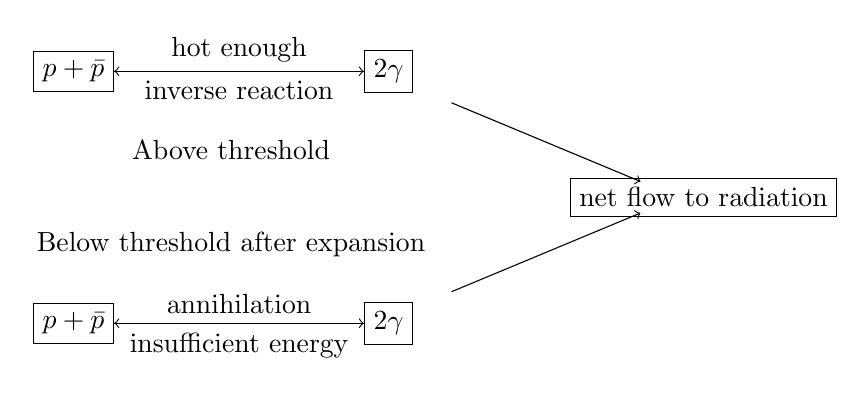
\begin{tikzpicture}[scale=1.0]
\node[draw,rectangle] (a1) at (-4,1.6) {$p+\bar p$};
\node[draw,rectangle] (b1) at (0,1.6) {$2\gamma$};
\draw[->] (a1) -- node[above] {hot enough} (b1);
\draw[->] (b1) -- node[below] {inverse reaction} (a1);

\node at (-2,0.6) {Above threshold};

\node[draw,rectangle] (a2) at (-4,-1.6) {$p+\bar p$};
\node[draw,rectangle] (b2) at (0,-1.6) {$2\gamma$};
\draw[->] (a2) -- node[above] {annihilation} (b2);
\draw[->,dashed] (b2) -- node[below] {insufficient energy} (a2);

\node at (-2,-0.6) {Below threshold after expansion};

\node[draw,rectangle] (c) at (4,0) {net flow to radiation};
\draw[->] (0.8,-1.2) -- (3.2,-0.2);
\draw[->] (0.8,1.2) -- (3.2,0.2);
\end{tikzpicture}
\caption{The ``one-way street'' logic of freeze-out. Above threshold, annihilation and inverse production can both occur. After expansion lowers photon energies, the inverse channel is thermally suppressed while annihilation still proceeds.}
\end{figure}

There is a simple count-bookkeeping example worth keeping in view. Suppose the initial proton and antiproton numbers are
\begin{equation}
N_p^{\mathrm{initial}} = N+\Delta,
\qquad
N_{\bar p}^{\mathrm{initial}} = N,
\end{equation}
with \(\Delta>0\) a tiny excess. One annihilation event changes the counts by
\begin{align}
N_p &\to N_p-1,\\
N_{\bar p} &\to N_{\bar p}-1,\\
N_\gamma &\to N_\gamma+2.
\end{align}
After all \(N\) available pairs have annihilated, one finds
\begin{equation}
N_p^{\mathrm{final}}=\Delta,
\qquad
N_{\bar p}^{\mathrm{final}}=0.
\end{equation}
That is the mathematical core of the story. Whatever the excess is, it survives, because it has no partners left to annihilate with.

The lecture then folds thermodynamics into the picture. The expansion is slow compared with microscopic reaction rates, so to a good approximation it is adiabatic. The precise conserved quantity is entropy, but for a thermal gas Susskind treats entropy as roughly the same thing as particle number, up to order-one factors. Thus the particles that disappear in annihilation are largely replaced by photons. That is why the present photon bath remembers the earlier annihilation history.

So we may infer the primordial asymmetry from the observed photon excess:
\begin{equation}
\frac{N_\gamma}{N_p} \sim 10^9\text{--}10^{10}.
\end{equation}
Equivalently, in the early hot soup there was only about one extra proton for every \(10^9\) proton-antiproton pairs. The present matter-filled universe is therefore not the fossil of a gross primordial asymmetry. It is the fossil of a very tiny one:
\begin{equation}
N_p-N_{\bar p} \neq 0,
\end{equation}
but only by roughly one part in a billion.

\section{Baryogenesis and the Sakharov Conditions}

The lecture now becomes a puzzle. If we begin with nearly equal amounts of matter and antimatter, why is there any residue at all?

\subsection{Question \& Answer}

\paragraph{Question.} Suppose the early universe was exactly symmetric,
\begin{equation}
N_p=N_{\bar p},
\end{equation}
and then simply cooled. Why can ordinary physics not generate a tiny extra proton population during cooling? And if not that, could the observed excess perhaps be only a statistical fluctuation?

\paragraph{Answer.} Cooling by itself is not enough. To create one extra proton, we must create positive electric charge, so electric neutrality forces us to create a negatively charged particle as well, say an electron. But more importantly, within the standard model at energies where it has been tested, one cannot create a proton without also creating an antiproton. The obstruction is not electric charge conservation. A proton plus an electron is electrically neutral. The obstruction is baryon-number conservation.

That is why the lecture insists on distinguishing
\begin{equation}
Q_{\mathrm{tot}}=0
\end{equation}
from
\begin{equation}
B=(N_p+N_n)-(N_{\bar p}+N_{\bar n}).
\end{equation}
Electric charge conservation is exact in the discussion. Baryon-number conservation is the empirical rule that blocks the naive mechanism.

The statistical alternative fails quantitatively. If there were no real bias in the laws, then random excesses would scale only as the square root of the total number of particles:
\begin{equation}
\Delta N_{\mathrm{stat}} \sim \sqrt{N}.
\end{equation}
Taking the observable universe at the rough lecture scale \(N\sim 10^{90}\) including photons gives
\begin{equation}
\sqrt{10^{90}} \sim 10^{45},
\end{equation}
whereas the actual proton count is of order \(10^{80}\). So the fluctuation estimate falls short by an absurd margin:
\begin{equation}
10^{45} \ll 10^{80}.
\end{equation}
The observed matter excess is therefore not a statistical accident of an otherwise unbiased freeze-out.

\begin{figure}[ht]
\centering

\includegraphics[width=0.72\textwidth]{lecture_06_figure_03.png}
\caption{Board state during the transition from the residual asymmetry \(N_p-N_{\bar p}\) to the developing list of conditions. The screenshot is useful mainly as documentary board evidence.}
\end{figure}

Once those escape routes are blocked, the lecture turns to the constructive answer: if the asymmetry is real, what must the laws of nature have allowed at very high temperature?

The answer is Sakharov's baryogenesis logic. The two key expressions preserved on the board are the symmetric starting point and the leftover asymmetry,
\begin{equation}
N_p=N_{\bar p},
\qquad
N_p-N_{\bar p}.
\end{equation}
To go from the first to the second, three ingredients are required.

\begin{figure}[ht]
\centering

\includegraphics[width=0.72\textwidth]{lecture_06_figure_04.png}
\caption{Asymmetry conditions and checklist on the board. The numbered text is reconstructed from the transcript rather than from the partial pixels alone.}
\end{figure}

\begin{enumerate}
\item \textbf{Violation of baryon number.} The laws must allow processes that change \(B\). Otherwise the net baryon number can never move away from zero.
\item \textbf{Violation of particle-antiparticle symmetry.} In the lecture this is first described as charge-conjugation asymmetry and later sharpened, correctly, to CP violation. Without such a bias, baryon-violating processes would create protons and antiprotons with equal average weight.
\item \textbf{Departure from thermal equilibrium.} If the universe stays in equilibrium, the particle-antiparticle asymmetry is driven back to zero.
\end{enumerate}

\begin{figure}[ht]
\centering
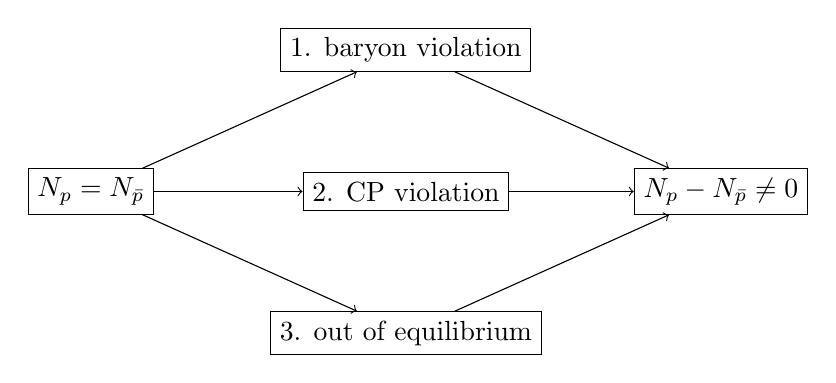
\begin{tikzpicture}[scale=1.0]
\node[draw,rectangle] (s) at (-4,0) {$N_p=N_{\bar p}$};
\node[draw,rectangle] (c1) at (0,1.8) {1. baryon violation};
\node[draw,rectangle] (c2) at (0,0) {2. CP violation};
\node[draw,rectangle] (c3) at (0,-1.8) {3. out of equilibrium};
\node[draw,rectangle] (f) at (4,0) {$N_p-N_{\bar p}\neq 0$};

\draw[->] (s) -- (c1);
\draw[->] (s) -- (c2);
\draw[->] (s) -- (c3);
\draw[->] (c1) -- (f);
\draw[->] (c2) -- (f);
\draw[->] (c3) -- (f);
\end{tikzpicture}
\caption{Minimal logical reconstruction of the board discussion: a symmetric starting point can tilt into a nonzero asymmetry only if all three Sakharov conditions are available.}
\end{figure}

The lecture presents this not as a theorem proved from first principles on the spot, but as a remarkably robust structure. If these conditions hold at sufficiently high temperature, then a tiny leftover asymmetry is not unnatural. If they do not hold, the asymmetry is extraordinarily hard to generate.

\section{Clarifications at the Edge of What We Know}

The final third of the lecture is a sequence of clarifications about what is known, what is inferred, and what remains conjectural.

First comes the relation between CP, time reversal, and equilibrium. The relevant exact statement is not charge conjugation by itself but the CPT theorem, built into relativistic quantum field theory. Very roughly: if we replace particles by antiparticles and simultaneously reverse time, the theory remains invariant. Why then is this relevant to baryogenesis? Because in thermal equilibrium a movie run backward looks like a movie run forward. If the system does not distinguish past from future at the microscopic level, then CPT collapses back into an effective particle-antiparticle symmetry for the equilibrium state. That is the lecture's reason for insisting that equilibrium is fatal to a persistent matter excess. A hot static pot cannot keep \(N_p\) different from \(N_{\bar p}\).

What is needed is not CPT violation but nonequilibrium. That distinction is crucial. The universe can have a definite time-directed history, namely expansion, without the underlying equations failing to admit the time-reversed history as another possible solution. Condition 3 is therefore
\begin{equation}
\text{out of equilibrium},
\end{equation}
not a violation of the CPT theorem.

Second comes the empirical status of baryon-number violation. The lecture is explicit: this is the question mark. We have never directly observed a reaction that changes the net baryon number. Yet there are strong reasons to think such processes may exist at very high temperature, while becoming fantastically improbable at low energy. That is why proton decay is so important. If baryon number is not exact, then a proton ought in principle to be able to decay, but perhaps with an immense lifetime.

The lecture quotes this scale in the way one expects from a board lecture: ordinary particle reactions happen on absurdly tiny time scales, but the proton must live at least as long as the age of the universe, and in fact far longer. The cited experimental lower bound is of order
\begin{equation}
\tau_p \gtrsim 10^{34}\ \text{years},
\end{equation}
at the level of the lecture's discussion. Large underground water detectors search for exactly this kind of event. So far, nothing.

Third comes the role of gravity. Gravity is not important because the direct gravitational interaction between elementary particles is large; it is negligible for the particle-physics bookkeeping. Gravity matters in two other ways. One is cosmological: without Einsteinian expansion there would be no departure from equilibrium on cosmic scales. The second is the black-hole thought experiment. If a baryon-rich star collapses into a black hole and later evaporates mostly into thermal radiation, then it becomes very difficult to believe that baryon number can remain an exact conservation law forever. This is not an observed baryon-violating process in the laboratory, but it is strong theoretical pressure against exact baryon conservation.

Electric charge is different. A charged black hole cannot simply forget its charge, because the electric flux lines remain tied to infinity. That is why the lecture treats electric charge as exact while treating baryon number as provisional.

\paragraph{Neutron coda.} The lecture ends with a short side discussion of neutrons, and it is worth keeping only the central point. Neutron beta decay,
\begin{equation}
n \to p + e^- + \bar\nu,
\end{equation}
does \emph{not} violate baryon number. The neutron carries the same baryon number as the proton. A free neutron decays because its mass is slightly larger than that of the final state. In very rough threshold language,
\begin{equation}
m_n \gtrsim m_p + m_e + m_\nu.
\end{equation}
The available energy is small, and that small phase space helps explain the long lifetime of the free neutron. When the neutron is bound inside a nucleus, binding energy can make decay kinematically unavailable. That is why bound neutrons can be stable even though free neutrons are not:
\begin{equation}
M_{\mathrm{bound}} \approx m_n + m_p - \frac{E_{\mathrm{bind}}}{c^2}.
\end{equation}
This coda is secondary to the baryogenesis story, but it serves the lecture's larger purpose: to separate a baryon-conserving weak decay from the genuinely hypothetical baryon-violating processes that baryogenesis would require.

\section{Summary}

The lecture begins with visibility and ends with asymmetry. Looking outward takes us to last scattering, and last scattering leads us to an earlier, hotter plasma in which pair creation was commonplace. Reversing the movie then shows how annihilation and freeze-out leave behind photons plus a tiny net residue of matter. The observed ratio
\[
\frac{N_\gamma}{N_p}\sim 10^9\text{--}10^{10}
\]
tells us that the primordial excess was only about one part in a billion.

From there the logic becomes sharp. Cooling by itself cannot generate the asymmetry within tested particle physics, and statistical fluctuations are far too small. The lecture therefore lands on Sakharov's three conditions: baryon-number violation, CP violation, and nonequilibrium. Of these, the last two are well motivated by known physics, while the first remains the decisive missing empirical piece. That is the epistemic texture of the lecture: the structure is compelling, the scale is plausible, but baryogenesis is still a story whose most important experimental confirmation has not yet been seen.